\section[py]{\cpp and python}

\subsection[module]{Writing a module}

\begin{frame}[fragile]
  \frametitle{How to build a python 3 module around \cpp code}
  \begin{block}{\cpp code : mandel.hpp}
    \begin{cppcode*}{}
      int mandel(Complex const & a);
    \end{cppcode*}
  \end{block}
\end{frame}

\begin{frame}[fragile]
  \frametitle{Basic Module(1) : wrap your method}
  \begin{block}{mandelModule.cpp - see code/python exercise}
    \begin{cppcode*}{}
      #include <Python.h>
      #include "mandel.hpp"
      PyObject * mandel_wrapper(PyObject * self,
                                PyObject * args) {
        // Parse Input
        float r, i;
        if (!PyArg_ParseTuple(args, "ff", &r, &i))
          return NULL;
        // Call C++ function
        int result = mandel(Complex(r, i));
        // Build returned objects
        return PyLong_FromLong(result);
      }
    \end{cppcode*}
  \end{block}
\end{frame}

\begin{frame}[fragile]
  \frametitle{Basic Module(2) : create the python module}
  \begin{block}{mandelModule.cpp - see code/python exercise}
    \begin{cppcode*}{}
      // declare the modules' methods
      PyMethodDef mandelMethods[] = {
          {"mandel", mandel_wrapper, METH_VARARGS,
          "computes nb of iterations for mandelbrot set"},
          {NULL, NULL, 0, NULL}
      };
      // declare the module
      struct PyModuleDef mandelModule = {
        PyModuleDef_HEAD_INIT,
        "mandel", NULL, -1, mandelMethods
      };
      PyMODINIT_FUNC PyInit_mandel(void) {
        return PyModule_Create(&mandelModule);
      }
    \end{cppcode*}
  \end{block}
\end{frame}

\begin{frame}[fragile]
  \frametitle{Basic Module(3) : use it}
  \begin{block}{First compile the module}
    \begin{itemize}
    \item as a regular shared library
    \item with '-I \$(PYTHON\_INCLUDE)'
    \end{itemize}
  \end{block}
  \begin{block}{mandel.py - see code/python exercise}
    \begin{minted}[gobble=4]{python}
      from mandel import mandel
      v = mandel(0.7, 1.2)
    \end{minted}
  \end{block}
\end{frame}


\subsection[C]{Marrying \cpp and C}

\begin{frame}[fragile]
  \frametitle{A question of mangling}
  \begin{block}{Mangling}
    the act of converting the name of variable or function to a symbol name in the binary code
  \end{block}
  \begin{block}{C versus \cpp symbol names}
    \begin{itemize}
    \item C uses bare function name
    \item \cpp allows overloading of functions by taking the signature into account
    \item so \cpp mangling has to contain signature
    \end{itemize}
  \end{block}
\end{frame}

\begin{frame}[fragile]
  \frametitle{C mangling}
  \begin{exampleblock}{Source : file.c}
    \begin{cppcode*}{}
      float sum(float a, float b);
      int square(int a);
      // won't compile : conflicting types for ‘square’
      // float square(float a);
    \end{cppcode*}
  \end{exampleblock}
  \begin{block}{Binary symbols : file.o}
    \begin{minted}[gobble=4]{shell}
      # nm file.o
      000000000000001a T square
      0000000000000000 T sum
    \end{minted}
  \end{block}
\end{frame}

\begin{frame}[fragile]
  \frametitle{\cpp mangling}
  \begin{exampleblock}{Source : file.cpp}
    \begin{cppcode*}{}
      float sum(float a, float b);
      int square(int a);
      // ok, signature is different
      float square(float a);
    \end{cppcode*}
  \end{exampleblock}
  \begin{block}{Binary symbols : file.o}
    \begin{minted}[gobble=4]{shell}
      # nm file.o
      0000000000000000 T _Z3sumff
      000000000000002a T _Z6squaref
      000000000000001a T _Z6squarei
    \end{minted}
  \end{block}
\end{frame}

\begin{frame}[fragile]
  \frametitle{Forcing C mangling in \cpp}
  \begin{block}{extern ``C''}
    These functions will use C mangling :
    \begin{cppcode*}{gobble=1}
      extern "C" {
        float sum(float a, float b);
        int square(int a);
      }
    \end{cppcode*}
  \end{block}
  \pause
  You can now call these \cpp functions from C code
  \pause
  \begin{alertblock}{Limitations}
    \begin{itemize}
    \item no \cpp types should go out
    \item no exceptions either (use noexcept here)
    \item member functions cannot be used
      \begin{itemize}
      \item they need to be wrapped one by one
      \end{itemize}
    \end{itemize}
  \end{alertblock}
\end{frame}

\subsection[ctypes]{The ctypes module}

\begin{frame}[fragile]
  \frametitle{The ctypes python module}
  \begin{block}{From the documentation}
    \begin{itemize}
    \item provides C compatible data types
    \item allows calling functions in DLLs or shared libraries
    \item can be used to wrap these libraries in pure Python
    \end{itemize}
  \end{block}
\end{frame}

\begin{frame}[fragile]
  \frametitle{ctypes : usage example}
  \begin{block}{\cpp code : mandel.hpp}
    \begin{cppcode*}{}
      int mandel(Complex const & a);
    \end{cppcode*}
  \end{block}
  \begin{block}{``C'' code : mandel\_cwrapper.hpp}
    \begin{cppcode*}{}
      extern "C" {
        int mandel(float r, float i) {
          return mandel(Complex(r, i));
        };
      }
    \end{cppcode*}
  \end{block}
  \begin{exampleblock}{calling the mandel library}
    \begin{minted}[gobble=4]{python}
      from ctypes import *
      libmandel = CDLL('libmandelc.so')
      v = libmandel.mandel(c_float(0.3), c_float(1.2))
    \end{minted}
  \end{exampleblock}
\end{frame}

\begin{frame}
  \frametitle{Marrying \cpp and python}
  \begin{alertblock}{Exercise Time}
    \begin{itemize}
    \item go to code/python
    \item look at the original python code mandel.py
    \item time it (`time python3 mandel.py`)
    \item look at the code in mandel.hpp/cpp
    \item look at the python module mandel\_module.cpp
    \item compile and modify mandel.py to use it
    \item see the gain in time
    \item look at the C wrapper in mandel\_cwrapper.cpp
    \item modify mandel.py to use libmandelc directly with ctypes
    \end{itemize}
  \end{alertblock}
  \tiny Note : you may have to add '.' to LD\_LIBRARY\_PATH and PYTHONPATH
\end{frame}

\subsection[cppyy]{The cppyy project}

\begin{frame}
  \frametitle{Automatic Python-C++ bindings}
  \begin{block}{The {\color{blue!50!white} \href{https://cppyy.readthedocs.io}{cppyy}} project}
    \begin{itemize}
    \item originated from the ROOT project
    \item still young, version 1.0 from Mid 2018
    \item but very active,  current version 2.1.0
    \item extremely powerful for interfacing \cpp and python
    \end{itemize}
  \end{block}
  \begin{block}{How it works}
    \begin{itemize}
    \item uses Just in Time compilation through {\color{blue!50!black} \href{https://github.com/vgvassilev/cling}{cling}}
      \begin{itemize}
      \item an interactive \cpp interpreter
      \end{itemize}
    \end{itemize}
  \end{block}
\end{frame}

\begin{frame}
  \frametitle{cppyy crash course(1)}
  Shamelessly copied from the cppyy documentation
  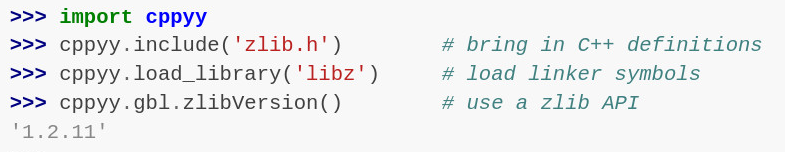
\includegraphics[width=.8\textwidth]{cppyy2.png}
  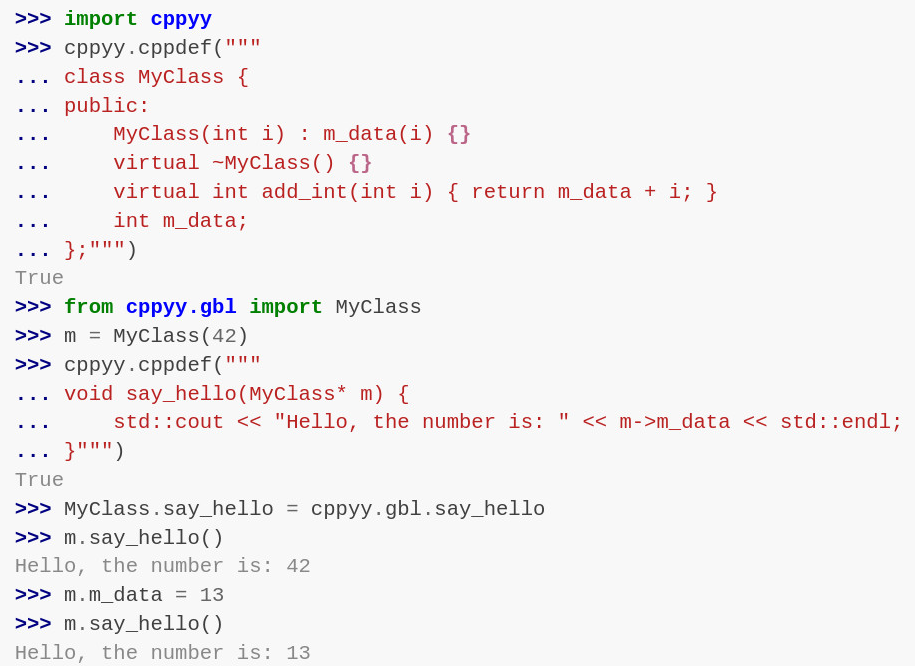
\includegraphics[trim={0 3.2cm 0 0},clip,width=\textwidth]{cppyy.png}
\end{frame}

\begin{frame}
  \frametitle{cppyy crash course(1)}
  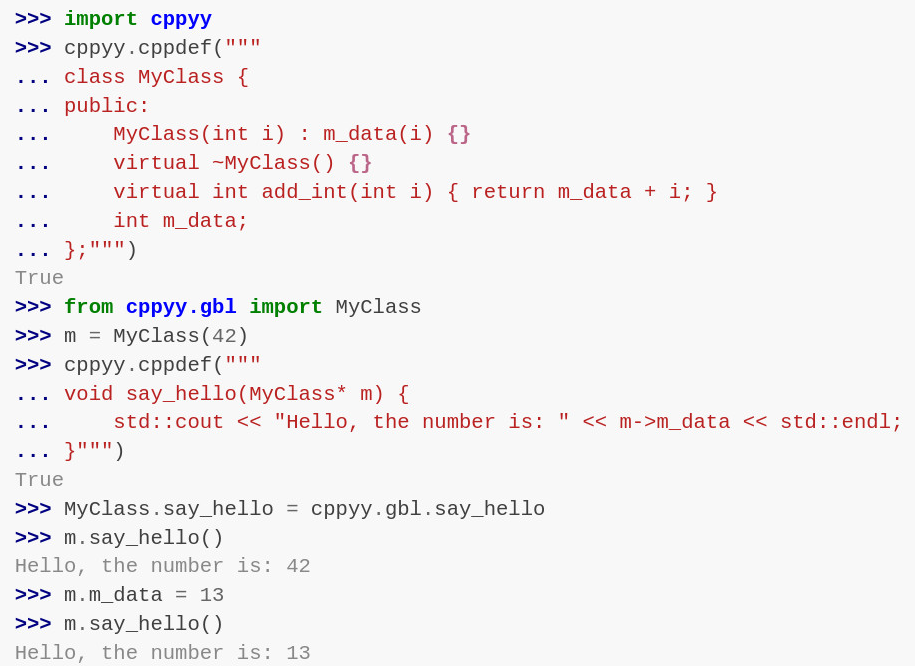
\includegraphics[trim={0 0 0 2.45cm},clip,width=\textwidth]{cppyy.png}
\end{frame}
